\section{Preliminaries}
\label{sec:preliminaries}

We adopt Canetti's formulation of ``real world'' notion of protocol execution \cite{JC:Canetti00,EPRINT:Canetti00} to model the computation for multi-party protocols.
%
The environment \Z provides input to parties that execute the protocol $\Pi$.
%
The adversary \adv is a single entity that controls all corrupted parties; and \adv is both ``adaptive'' (i.e., take control of parties on the fly) and ``rushing'' (i.e., \adv can observe honest parties' actions and then react).
%
We describe the ``resources'' that may be available to the protocol instances (e.g., access to a ``diffuse'' channel) as \emph{ideal functionalities} in the terminology of~\cite{EPRINT:Canetti00}.

\subsection{Drifting Clocks and Clock Synchronization}
\label{subsec:drifting-clocks-and-synchronization}

We assume the existence of ``nominal time'' (cf.~\cite{EC:BGKRZ21,TCC:GarKiaShe22}, also known as ``real time'' or ``Newtonian time'' \cite{JCSS:DHS86}), which is not directly observable by protocol participants.
%
Following the traditional assumption in distributed computing that each party is equipped with a physical clock, whose output is a real-valued function of nominal time, in this paper we consider the \textbf{drifting clock} model.
%
Specifically, honest parties possess physical clocks with a bounded rate of drift from nominal time (\cref{fig:drifting-clocks}) --- i.e., an honest physical clock stays within a \emph{linear envelope} of nominal time.\footnote{A function $f: \mathbb{R} \rightarrow \mathbb{R}$ is within a $(U, L)$-linear envelope if and only if it holds that $L \cdot x - c \leq f(x)\leq U \cdot x + c$, where $c$ is a constant and $x \in \mathbb{R}^+$.}
%
We use \clockDrift to denote the bound on the rate of honest physical clocks.
% 
Formally, for any nominal time $u > v$ and an honest physical clock $D$, it holds that
%
\[ (1 + \clockDrift)^{-1} (u - v) \le D(u) - D(v) \le (1 + \clockDrift) (u - v). \]

\begin{figure}[ht]
    \centering
    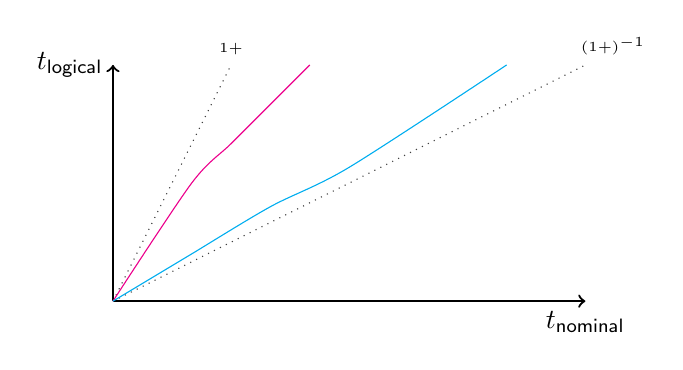
\begin{tikzpicture}
        \draw[->, thick] (0, 0) -- (6, 0) node[below] {$t_{\mathsf{nominal}}$};
        \draw[->, thick] (0, 0) -- (0, 3) node[left] {$t_{\mathsf{logical}}$};

        \draw[dotted, color = darkgray] (0, 0)--(6, 3) node[above, color = black, xshift=1em] {\tiny $(1 + \clockDrift)^{-1}$};
        \draw[dotted, color = darkgray] (0, 0)--(1.5, 3) node[above, color = black] {\tiny $1 + \clockDrift$};

        \draw[opacity=0]  (0,0) -- (1,1) -- (1.5, 2) -- (2, 2.5)  -- (3, 3);

        \draw [magenta] plot [smooth] coordinates { (0,0) (1,1.5) (1.5, 2) (2, 2.5) (2.5, 3)};

        \draw [cyan] plot [smooth] coordinates { (0, 0) (0.5, 0.3) (1, 0.6) (2, 1.2) (3, 1.7) (5, 3)};
    \end{tikzpicture}

    \caption{An illustration of drifting clocks within a $(0.5, 2)$-linear envelope (i.e., $\clockDrift = 1$). Without clock synchronization, two clocks (illustrated in magenta and cyan, respectively) deviate from each other unboundedly.}
    \label{fig:drifting-clocks}
\end{figure}


Note that time in the drifting clock model are real values, while our protocol execution model divides time into discrete integer-numbered steps.
%
In order to ``insert'' real-valued time into this structure, we model drifting local clocks as \funcDriftingClock, derived from the global clock functionality in~\cite{TCC:KMTZ13}.
%
In \funcDriftingClock, nominal time is defined by the number of times that the clock functionality moves forward the time-step variable $\tau$ (which is an internal variable and is unknown to the parties).
%
Instead of directly receiving the time from \funcDriftingClock, parties receive ``ticks'' from \funcDriftingClock which indicates that they should advance their local round number.
%
\funcDriftingClock advances the nominal time when all (honest) participants claim they have finished their computation in the current round.
%
Additionally, \funcDriftingClock allows the adversary to ``push'' or ``stall'' honest clocks, as long as these operations do not violate the \clockDrift-bounded linear envelope assumption.
%
We present \funcDriftingClock in~\cref{functionality:drifting-clock}.

\begin{remark}
    As opposed to the classical distributed computing setting (cf.~\cite{JACM:DwoLynSto88}) where rounds/time steps are defined as intervals of equal length in the view of an external real-time clock, in our model \funcDriftingClock does not guarantee that rounds/time steps are of equal duration.
    %
    In fact, the notions of `time' and `duration' are not defined in the UC setting.
    %
    Yet, our model shows the same effect in restricting local clock counters staying in a bounded linear envelope with respect to the nominal clock counter; moreover, the same amount of computation is carried out per local time counter increment --- which means that in the same window of nominal time, a faster CPU will solve more PoWs than a slower one.
\end{remark}

\begin{cccFunctionality}
    {\funcDriftingClock}
    {drifting-clock}
    {The drifting global clock.}

    This functionality maintains state variables as follows.

    \addtocounter{table}{-1}
    \begin{tabularx}{.9\textwidth}{c X}
        \toprule[.3mm]
        \textbf{State Variable}
         & \textbf{Description}
        \\ \midrule[.3mm]
        $\clockDrift \gets 0$
         & The bound on clock drifts.
        \\ \midrule
        $\partyset \gets \emptyset$
         & The set of registered parties $\party = (\pid, \sid)$.
        \\ \midrule
        $F \gets \emptyset$
         & The set of registered functionalities (together with their session identifier).
        \\ \midrule
        $\tau_\sid \gets 0$
         & The nominal-time variable for session \sid.
        \\ \midrule
        $d_\party \gets 0$
         & The clock-update variable for $\party = (\pid, \sid) \in \partyset$.  $d_\party$ is set to $1$ after \party finishes a round.
        \\ \midrule
        $b_\party \gets 1$
         & The tick-budget variable for $\party = (\pid, \sid) \in \partyset$.
        \\ \midrule
        $d(\F, \sid) \gets 0$
         & The clock-update variable for $(\F, \sid) \in F$.
        \\ \bottomrule[.3mm]
    \end{tabularx}

    \paragraph{Setting the drift:}
    %
    \begin{cccItemize}[nosep]
        \item Upon  receiving $(\textsc{set-drift}, \sid, r)$ from the adversary \adv, \textbf{if} \textsc{set-drift} has never been received then set $\clockDrift = r$. Return $(\textsc{set-drift}, \sid, \ok)$ to \adv.
    \end{cccItemize}

    \paragraph{Clock capabilities:}
    %
    \begin{cccItemize}[nosep]
        \item Upon receiving $(\textsc{clock-update}, \sid_C)$ from some party $\party \in \partyset$ set $d_\party \gets 1$ and $b_\party \gets b_\party - 1$; execute \textit{Time-Update} and forward $(\textsc{clock-update}, \sid_C , \party)$ to \adv.

        \item Upon receiving $(\textsc{clock-update}, \sid_C)$ from some functionality \F in a session \sid such that $(\F, \sid) \in F$ set $d(\F, \sid) \gets 1$, execute \emph{Time-Update} and return $(\textsc{clock-update},\allowbreak \sid_C, \F)$ to this instance of \F.

        \item Upon receiving $(\textsc{clock-forward}, \sid_C , \party)$ from \adv where $\party \in \partyset$, if $d_\party = 0$ or it is about to violate the \clockDrift-bounded linear envelope on \party, ignore the message.
        %
        Otherwise, update $d_\party = 0$ and $b_\party \gets b_\party + 1$; return $(\textsc{clock-forward-ok}, \sid_C , \party)$ to \adv.

        \item Upon receiving $(\textsc{clock-backward}, \sid_C , \party)$ from \adv where $\party \in \partyset$, if $d_\party = 0$ or it is about to violate the \clockDrift-bounded linear envelope on \party, ignore the message.
        %
        Otherwise, update $b_\party \gets b_\party - 1$; return $(\textsc{clock-backward-ok}, \sid_C , \party)$ to \adv.

        \item Upon receiving $(\textsc{clock-tick}, \sid_C)$ from any participant \party --- including the environment on behalf of a party --- or the adversary on behalf of a corrupted party \party (resp. from any ideal---shared or local---functionality \F), execute procedure \textit{Time-Update}, return $(\textsc{clock-tick}, \sid_C, d_{\party})$ (resp. $(\textsc{clock-tick}, \sid_C, d_{(\F, \sid)})$) to the requestor (where \sid is the session id of the calling instance).

        \item Upon receiving $(\textsc{clock-read}, \sid_C)$ from the adversary or the wapper functionalities, return $(\textsc{clock-read},\sid_C, \tau_{\sid})$ to the requestor (where \sid is the session id of the calling instance).
    \end{cccItemize}

    \medskip\emph{Procedure Time-Update:}
    %
    For each session \sid do: If (i) $d_{(\func, \sid)} = 1$ for all $\func \in F$, and (ii) $d_\party = 1$ and $b_\party \le 0$ for all honest parties $\party = (\cdot, \sid) \in \partyset$, then update $\tau_\sid \gets \tau_\sid + 1$, $d_{(\func,\sid)} \gets 0$ and $b_\party \gets b_\party + 1$ for all parties $\party = (\cdot, \sid) \in \partyset$.
    %
    Additionally, for all parties $\party = (\cdot, \sid) \in \partyset$ with $b_\party > 0$, update $d_\party \gets 0$.
\end{cccFunctionality}


We adapt the traditional definition of the clock synchronization problem (cf.~\cite{JCSS:DHS86,JACM:SriTou87}) to our permissionless setting.
%
In~\cref{def:clock-properties}, we consider two properties, \emph{bounded skew} and \emph{accuracy}, that establish upper bounds \maxSkew and $\varGamma$ on honest clock skew and their deviation from the nominal time, respectively.

\begin{definition}
    [Clock Synchronization]
    \label{def:clock-properties}
    There exist constants $\maxSkew \in \mathbb{N}$, $\varGamma \in \mathbb{R}^+$ such that honest parties' logical clocks satisfy the following two properties:
    %
    \begin{cccItemize}[nosep]
        \item \emph{\bf Bounded skew (with parameter $\maxSkew \in \mathbb{N}$).}
        %
        Let $\round_1, \round_2$ be the reported logical clocks of two
        honest parties at any nominal time $r$.
        %
        Then $|\round_ 1 - \round_2| \le \maxSkew$.

        \item \emph{\bf Accuracy (with parameter $\varGamma \in \mathbb{R}^+$).}
        %
        Each honest party's logical clock stays in a $(U, L)$-linear envelope with respect to the nominal time $r$, where $U = 1 + \varGamma$ and $L = 1 / (1 + \varGamma)$.
    \end{cccItemize}
\end{definition}

\subsection{Random Oracle, Network and Adversarial Model}
\label{subsec:ro-network-corruption}

\paragraph{Random oracle.}
%
By convention, we model the cryptographic hash function $H$ with output in $\{0, 1\}^\kappa$ (which is used to generate proofs of work [PoWs]) as a random oracle \funcRO~\cite{CCS:BelRog93}.

\input{functionalities/random-oracle}

We express our honest majority condition in terms of computational power, measured in particular by the number of queries to the RO that the parties are allowed to make per \emph{nominal time-step}, as opposed to expressing it by the number of parties (i.e., the ``flat'' model where parties are assumed to have equal computational power---cf.~\cite{EC:GarKiaLeo15}).

\begin{definition}[Honest Majority]
    Let $h_r, t_r$ denote the number of \emph{alert} and \emph{non-alert} random oracle queries at \emph{nominal} time $r$, respectively.
    %
    Then, for all $r \in \mathbb{N}$, it holds that $h_r > t_r$.
\end{definition}

This restriction on the number of RO queries is captured by a wrapper functionality on \funcRO via counting the number of \emph{alert} and other queries (see below) per nominal-time step.
%
The adversary is allowed to dynamically and adaptively determine the number of alert random oracle queries per nominal-time step, as long as it does not violate the restrictions imposed by the $(\gamma, s)$-respecting environment (see~\cref{def:respecting-environment} in the sequel).

\begin{cccFunctionality}
    {\wrapper{\funcRO}}
    {random-oracle-wrapper}
    {The random oracle wrapper.}

    This functionality maintains state variables as follows.

    \addtocounter{table}{-1}
    \begin{tabularx}{.9\textwidth}{c  X}
        \toprule[.3mm]
        \textbf{State Variable}
         & \textbf{Description}
        \\ \midrule[.3mm]
        $\partyset \gets \emptyset$
         & The set of registered parties; the current set of corrupted parties is denoted by $\partyset'$.
        \\ \midrule
        $\tau \gets 0$
         & The (real-time) clock tick counter.
        \\ \midrule
        $h_\tau$
         & An upper bound which restricts the \func-evaluations of all alert parties at time $\tau$.
        \\ \midrule
        $q_\honestPartySet, q_\adv \gets 0$
         & The alert/adversary evaluation counter.
        \\ \bottomrule[.3mm]
    \end{tabularx}

    \paragraph{Pre-mining attack handling (executed only if $\tau = 0$):}
    %
    \begin{cccItemize}[nosep]
        \item Upon receiving $(\textsc{eval}, \sid, x)$ from \adv on behalf of a corrupted party $P \in \partyset'$, forward the request to \funcRO and return to \adv whatever \funcRO returns.

        \item Upon receiving $(\textsc{Retrieved}, \sid)$ from \funcCRS, set $\tau = 1$.
    \end{cccItemize}

    \paragraph{Relaying inputs to the random oracle:}
    %
    \begin{cccItemize}[nosep]
        \item Upon receiving $(\textsc{eval}, \sid, x)$ from \adv on behalf of a corrupted party $P \in \partyset'$ or a de-synchronized party \party, first execute \textit{Round Reset}, then do the following.
        %
        \begin{cccEnum}[nosep]
            \item Set $q_\adv \gets q_\adv + 1$.
            \item \textbf{If} $q_\adv \le h_\tau$ \textbf{then} forward the request to \funcRO and return to \adv whatever \funcRO returns.
        \end{cccEnum}

        \item Upon receiving $(\textsc{eval}, \sid, x)$ from an alert party \party, first execute \textit{Round Reset}, then do the following.
        %
        \begin{cccEnum}[nosep]
            \item Set $q_\honestPartySet \gets q_\honestPartySet + 1$.
            \item \textbf{If} $q_\honestPartySet \le h_\tau$ \textbf{then} forward the request to \funcRO and return to \party whatever \funcRO returns.
            \item \textbf{If} $q_\honestPartySet \ge h_\tau$ \textbf{then} send $(\textsc{clock-update}, \sid_C)$ to \funcDriftingClock.
        \end{cccEnum}
    \end{cccItemize}

    \paragraph{Corruption handling:}
    %
    \begin{cccItemize}[nosep]
        \item Upon receiving $(\textsc{corrupt}, \sid, \party)$ from the adversary, set $\partyset' \gets \partyset' \cup \party$.
    \end{cccItemize}

    \medskip\emph{Procedure Round-Reset:}
    %
    Send $(\textsc{clock-read}, \sid_C)$ to \funcDriftingClock and receive $(\textsc{clock-read}, \allowbreak \sid_C, \tau')$ from \funcDriftingClock. If $|\tau - \tau' | > 0$, then do the following.
    %[
    \begin{cccEnum}[nosep]
        \item Set $q_\honestPartySet, q_\adv \gets 0$ and $\tau \gets \tau'$.

        \item Send $(\textsc{next-round})$ to \adv and receive as response $(\textsc{next-round}, h^*_{\tau'})$.
        %
        \textbf{If} $(h_1, h_2, \ldots, h'_{\tau'})$ is $(\gamma, s)$-respecting (\cref{def:respecting-environment}) \textbf{then} set $h_{\tau'} = h'_{\tau'}$; \textbf{else} set $h_{\tau'} = h_{\tau' - 1}$.
    \end{cccEnum}
\end{cccFunctionality}


In addition, pre-mining attack prevention is captured by restricting the number of adversarial queries after a fresh CRS is released (which we model as \funcCRS).

\begin{cccFunctionality}
    {\funcCRS}
    {CRS}
    {The common reference string.}

    The functionality is parameterized by a distribution $\mathcal{D}$.

    \begin{cccItemize}[noitemsep]
        \item \textbf{Retrieve.} Upon receiving $(\textsc{Retrieve}, \sid)$ from some party \party (or from \adv on behalf of a corrupted \party), do the following:
        %
        \begin{cccEnum}[nosep]
            \item If activated for the first time, choose a value $d \gets \mathcal{D}$, and send $(\textsc{Retrieved}, \sid)$ to \wrapper{\funcRO} and \wrapper{\funcDiffuse}.

            \item Return $(\textsc{Retrieve}, d)$ to \party.
        \end{cccEnum}
    \end{cccItemize}
\end{cccFunctionality}

\paragraph{The bounded-delay network.}
%
Regarding communication amongst parties, we consider a peer-to-peer diffusion network, where the message dissemination has an (unknown) \delay-bounded delay.
%
In more detail, an honest message sent at time $t$ will be received by all other honest parties before time $t + \delay$; regarding messages sent by the adversary, if $t$ is the earliest time such that at least one honest party receives those messages, they are guaranteed to be delivered to all honest parties before time $t + \delay$ (i.e., honest parties keep ``echoing'' messages).

We capture this communication network with \funcDiffuse (\cref{functionality:diffuse}).
%
Recall that existing diffuse functionalities (cf.~\cite{C:BMTZ17}) model delays in the following manner:
%
There is a fetch counter per message per recipient such that when each time an honest party \party is activated and received a new tick from the clock, \party fetches on \funcDiffuse which reduces counters by $1$ for all messages delivering to \party; she then receives a subset of those messages with counters reset to $0$.
%
Regarding the adversary, he can increase the counter for each message and recipient for up to \delay in accumulation (as well as swapping the order of messages).

By convention, different types of messages are diffused by different functionalities, and we write $\funcDiffuse^{\textsf{bc}}$, $\funcDiffuse^{\textsf{input}}$, $\funcDiffuse^{\textsf{tx}}$ to denote the network for chains, input blocks and transactions.

\input{functionalities/diffuse}

We highlight that such mechanism does \emph{not} work in our drifting clock model with \funcDriftingClock (it only works with a global clock where parties proceed with the same speed).
%
This is because, when modeling delays via fetches on the diffuse functionality, honest parties that experience relatively fast local rounds would request more \textsc{fetch} commands than the slow ones in the same window of nominal time --- i.e., if an honestly-sent message is set the same delay for two parties then it delivers to the fast one earlier; yet our goal is to model delays measured in the perspective of the nominal time (regardless of parties' local understanding of time).

We resolve this issue by introducing a new wrapper on \funcDiffuse (\cref{functionality:wrapper-diffuse}) that restricts the adversary's capability to delay messages for up to \delay nominal time.
%
After registering on \funcDriftingClock to learn the nominal time ticks, the wrapper functionality dynamically relays parties' \textsc{fetch} request to \funcDiffuse so that in every nominal-time step, exactly one fetch operation is relayed to \funcDiffuse for each honest party (even if that honest party receives multiple ticks from \funcDriftingClock).
%
Meanwhile, for each party \party that proceeds slowly and may not activate in a given nominal time, the wrapper queries \funcDiffuse on behalf of \party, buffers the response messages and delivers them to \party upon the next time \party interacts with the wrapper.

\begin{cccFunctionality}
    {\wrapper{\funcDiffuse}}
    {wrapper-diffuse}
    {The wrapper of diffuse network.}

    This functionality maintains state variables as follows.

    \addtocounter{table}{-1}
    \begin{tabularx}{.9\textwidth}{c  X}
        \toprule[.3mm]
        \textbf{State Variable}
         & \textbf{Description}
        \\ \midrule[.3mm]
        $\partyset \gets \emptyset$
         & The set of registered parties; the current set of corrupted parties is denoted by $\partyset'$.
        \\ \midrule
        $\tau \gets 0$
         & The (real-time) clock tick counter.
        \\ \midrule
        $\mathsf{fetch}(\party, \tau) \gets 0$
         & The fetch variable for party \party at nominal time $\tau$.
        \\ \midrule
        $\mathsf{buffer}_\party \gets []$
         & The fetch buffer for party \party.
        \\ \bottomrule[.3mm]
    \end{tabularx}

    \paragraph{Relaying inputs to the diffuse network:}
    %
    \begin{cccItemize}[nosep]
        \item Upon receiving $(\textsc{diffuse}, \sid, m)$ from \adv on behalf of some corrupted $\party \in \partyset'$, parse $m$ as blocks $\block_1, \ldots, \block_n$.
        %
        For each $\block_i$, if $\block_i$ has not been queried to \funcRO, send $(\textsc{eval}, \sid, \block_i)$ from a corrupted party.

        \item Upon receiving $(\textsc{fetch}, \sid)$ from an honest party \party, if $\mathsf{fetch}(\party, \tau) = 1$ ignore this request.
        %
        Otherwise, execute the following:
        %
        \begin{cccEnum}[nosep]
            \item Forward $(\textsc{fetch}, \sid)$ to \funcDiffuse and recevie as response $\vec{M}$, return $\mathsf{buffer}_\party \concat \vec{M}$.
            \item Set $\mathsf{buffer}_\party \gets []$ and $\mathsf{fetch}(\party, \tau) \gets 1$.
        \end{cccEnum}
    \end{cccItemize}

    \paragraph{Corruption handling:}
    %
    \begin{cccItemize}[nosep]
        \item Upon receiving $(\textsc{corrupt}, \sid, \party)$ from the adversary, set $\partyset' \gets \partyset' \cup \party$.
    \end{cccItemize}

    \medskip\emph{Procedure Round-Reset:}
    %
    Send $(\textsc{clock-read}, \sid_C)$ to \funcDriftingClock and receive $(\textsc{clock-read}, \allowbreak \sid_C, \tau')$ from \funcDriftingClock. If $|\tau - \tau' | > 0$, then do the following.
    %[
    \begin{cccEnum}[nosep]
        \item Set $\tau \gets \tau'$.

        \item  For each honest party $\party$ such that $\mathsf{fetch}(\party, \tau) = 0$, send $(\textsc{fetch}, \sid)$ to \funcDiffuse from \party and recevie as response $\vec{M}$, set $\mathsf{buffer}_\party \gets \mathsf{buffer}_\party \concat \vec{M}$.
        %
        For each honest party $\party$ such that $\mathsf{fetch}(\party, \tau) = 1$, set $\mathsf{fetch}(\party, \tau) \gets 0$.

        \item Send $(\textsc{clock-update}, \sid_C)$ to \funcDriftingClock.
    \end{cccEnum}
\end{cccFunctionality}


\paragraph{Dynamic availability and respecting environment.}
%
In order to apply a more fine-grained classification on protocol participants, we follow the treatment in~\cite{CCS:BGKRZ18} and classify parties into different types based on their accessible resources and synchronization states.
%
Specifically, a party is (i) \emph{operational} if she is registered with the random oracle \funcRO, and \emph{stalled} otherwise; (ii) \emph{online} if she is registered with the network \funcDiffuse, and \emph{offline} otherwise; (iii) \emph{time-aware} if she is registered with the drifting clock \funcDriftingClock, and \emph{time-unaware} otherwise; and (iv) \emph{synchronized} if she has been participated in the protocol for sufficiently long time and held ``synchronized state'' and ``synchronized time'' with other synchronized parties, and \emph{desynchronized} otherwise.

We define \emph{alert} parties based on the classification above.
%
Specifically, alert parties are those who have access to all the resources and are synchronized.
%
They are the core set of parties to carry out the protocol.

Next, we define a ``respecting environment'' in terms of the computational power (cf.~\cite{TCC:GarKiaShe22}) as opposed to number of parties (cf.~\cite{C:GarKiaLeo17,EPRINT:GarKiaLeo20}).
%
Our honest-majority assumption is that during the whole protocol execution, the alert computational power is higher than the adversarial one.
%
We restrict the environment so that the number of such queries will be bounded in a certain fashion.

\begin{definition} \label{def:respecting-environment}
    For $\gamma \in \mathbb{R}^+$ we call the sequence $(h_r)_{r \in [0, B)}$, where $B \in \mathbb{N}$, $(\gamma, s)$-respecting if for any set $S \subseteq [0, B)$ of at most $s$ consecutive integers, $\max_{r \in S} h_r \le \gamma \cdot \min_{r \in S} h_r$.
\end{definition}

\subsection{Blockchain Notation}

A block with target $T \in \mathbb{N}$ is a quadruple of the form $\block = \langle ctr, r, h, x \rangle$ where $ctr, r \in \mathbb{N}$, $h \in \{0, 1\}^{\kappa}$ and $x \in \{0, 1\}^*$.
%
A blockchain \chain is a (possibly empty) sequence of blocks; the rightmost block is denoted by \chainHead{\chain} (note $\chainHead{\varepsilon} = \varepsilon$).
%
These blocks are chained in the sense that if $\block_{i + 1} = \langle ctr, r, h, x \rangle$, then $h = H(\block_i)$.
%
We use \timestamp{\block} to denote the \emph{timestamp} of \block.
%
We denote by \chainPrefixUB{\chain}{t} the chain resulting from ``pruning'' the least number of rightmost blocks so that all block timestamps are less than $t$.
%
Let $\parallelChains = \langle \chain_1, \chain_2, \ldots, \chain_m \rangle$ denote $m$ \emph{parallel} chains and $\parallelChains_j$ the $j$-th chain $\chain_j$ in \parallelChains.

Next, we introduce some basic string notation, which will be useful when describing our multi-chain-oriented PoW mechanism.
%
For a $\kappa$-bit string $s$, where $\kappa$ is the security parameter, we will use $s_i~(i \in [m])$ to denote the $i$-th bit of $s$, \stringSegment{s}{i}{m} to denote the $i$-th segment after $s$ is equally divided into $m$ segments---i.e., $\stringSegment{s}{i}{m} = s_{[(i - 1) * \kappa / m ]+ 1}, \ldots, s_{i * \kappa / m}$.
%
Further, we will write \stringRev{s} as the reverse of string $s$ (i.e., the string obtained by reversing the order of its bits), and use \stringSegmentRev{s}{i}{m} to denote the reverse of the $i$-th segment.

Finally, we introduce some array operations, following the notation in~\cite{JACM:DLPSW86}, that will be useful when describing the protocol.
%
Let $\mathbf{V} = (v_1, \ldots, v_n)$ be a real array of $n$ elements and denote $\tilde{\mathbf{V}} = (\tilde{v}_1, \ldots, \tilde{v}_n)$ the array after ordering $\mathbf{V}$ non-decreasingly.
%
We define the operations \textsf{reduce} and \textsf{select}.
%
Intuitively, \textsf{reduce} with parameter $\mathbf{V}$ and $\eta$ first orders $\mathbf{V}$ non-decreasingly and then ``trims'' the $\eta$ largest and $\eta$ smallest elements in $\tilde{\mathbf{V}}$; \textsf{select} with parameter $\mathbf{V}$ and $\eta$ first orders $\mathbf{V}$ non-decreasingly and then selects every first element of $\eta$ consecutive elements and forms them as a new array.
%
Formally,
%
\begin{equation} \label{eq:reduce-select}
    \mathsf{reduce}(\mathbf{V}, \eta) = (\tilde{v}_{\eta + 1}, \ldots, \tilde{v}_{n - \eta})
    ~~\text{and}~~
    \mathsf{select}(\mathbf{V}, \eta) = (\tilde{v}_1, \tilde{v}_{\eta + 1}, \tilde{v}_{2\eta + 1}, \ldots).
\end{equation}
%
Additionally, for an array $\mathbf{V}$, let $\mathsf{avg}(\mathbf{V})$ denote the average of its elements, and $\med(\mathbf{V})$ denote the median.

\subsection{Weak/Approximate Agreement}
\label{subsec:weak-approximate-agreement}

\paragraph{Weak agreement.}
%
A variant of Byzantine agreement --- \emph{Weak Agreement} -- relaxes the agreement property to allow some parties to output a special failing symbol $\bot$ while requiring all non-$\bot$ outputs being consistent \cite{JoA:Dolev82}.
%
This simple primitive has been widely used in building stronger notion of agreement (e.g., graded agreement).
%
We here provide the definition of Weak Agreement.

\begin{definition}
    [Weak Agreement]
    \label{def:weak-agreement}
    A protocol $\Pi$ implements Weak Agreement provided it satisfies the following two properties:
    %
    \begin{cccItemize}[nosep]
        \item \emph{\textbf{Weak Agreement}}: There exists $y \in \{0, 1\}$ such that all honest parties output $y_i \in \{ y, \bot \}$.

        \item \emph{\textbf{Validity}}: If all honest parties have the same input $b \in \{0, 1\}$, they all output $y_i = b$.
    \end{cccItemize}
\end{definition}

\paragraph{Approximate agreement.}
%
\emph{Approximate Agreement} (AA), formulated in~\cite{JACM:DLPSW86}, is a variant of the Byzantine agreement problem~\cite{JACM:PeaShoLam80,TOPLAS:LamShoPea82} in which processes start with arbitrary real values rather than Boolean values or values from some bounded range, and in which approximate, rather than exact, agreement is the desired goal.
%
In the classical distributed computing literature, AA has served as a fundamental building block to achieve clock synchronization (see, e.g.,~\cite{PODC:LunLyn84,PODC:MahSch85,PODC:LenLos22}).

Next, we present a definition of AA which captures adaptive security.
%
Conventionally, the goal is to let honest parties agree on outputs where the difference between any two of them is upper-bounded by a constant.
%
In this paper, we provide an alternate yet equivalent definition which asks for a ``concentration'' on the outputs compared with the inputs.
%
We denote $\epsilon$ as the ``quality'' of the agreement---i.e., the ratio between honest-input distance and output distance.

\begin{definition}
    [Approximate Agreement]
    \label{def:approximate-agreement}
    A protocol $\Pi$ is an $\epsilon$-secure protocol for Approximate Agreement provided it satisfies the following two properties:
    %
    \begin{cccItemize}[nosep]
        \item \emph{\textbf{$\epsilon$-Agreement}}: There is a round after which (i) any two honest parties hold inputs with difference at most $\ell$, and (ii) any two honest parties return outputs with difference at most $\epsilon \cdot \ell$ (where $0 < \epsilon < 1$) if queried by the environment.

        \item \emph{\textbf{Validity}}: The output returned by an honest party \party falls in the convex hull of the inputs of all parties at round $1$ that are honest at the round \party's output is produced.
    \end{cccItemize}
\end{definition}

